%% For double-blind review submission, w/o CCS and ACM Reference (max submission space)
\documentclass[sigplan,10pt,screen]{acmart}
\pagestyle{plain}
\pagenumbering{gobble}
%\documentclass[sigplan,review]{acmart}\settopmatter{printfolios=true,printccs=false}
%% For double-blind review submission, w/ CCS and ACM Reference
%\documentclass[sigplan,review,anonymous]{acmart}\settopmatter{printfolios=true}
%% For single-blind review submission, w/o CCS and ACM Reference (max submission space)
%\documentclass[sigplan,review]{acmart}\settopmatter{printfolios=true,printccs=false,printacmref=false}
%% For single-blind review submission, w/ CCS and ACM Reference
%\documentclass[sigplan,review]{acmart}\settopmatter{printfolios=true}
%% For final camera-ready submission, w/ required CCS and ACM Reference
%\documentclass[sigplan]{acmart}\settopmatter{}

\def\BibTeX{{\rm B\kern-.05em{\sc i\kern-.025em b}\kern-.08emT\kern-.1667em\lower.7ex\hbox{E}\kern-.125emX}}

%% Conference information
%% Supplied to authors by publisher for camera-ready submission;
%% use defaults for review submission.
\acmConference[CS 380C]{Compilers}{Fall 2019}{UT Austin}
%\acmYear{2018}
%\acmISBN{} % \acmISBN{978-x-xxxx-xxxx-x/YY/MM}
%\acmDOI{} % \acmDOI{10.1145/nnnnnnn.nnnnnnn}
\startPage{1}

%% Copyright information
%% Supplied to authors (based on authors' rights management selection;
%% see authors.acm.org) by publisher for camera-ready submission;
%% use 'none' for review submission.
\setcopyright{none}
%\setcopyright{acmcopyright}
%\setcopyright{acmlicensed}
%\setcopyright{rightsretained}
%\copyrightyear{2018}           %% If different from \acmYear

%% Bibliography style
%\bibliographystyle{ACM-Reference-Format}
%% Citation style
%\citestyle{acmauthoryear}  %% For author/year citations
%\citestyle{acmnumeric}     %% For numeric citations
%\setcitestyle{nosort}      %% With 'acmnumeric', to disable automatic
                            %% sorting of references within a single citation;
                            %% e.g., \cite{Smith99,Carpenter05,Baker12}
                            %% rendered as [14,5,2] rather than [2,5,14].
%\setcitesyle{nocompress}   %% With 'acmnumeric', to disable automatic
                            %% compression of sequential references within a
                            %% single citation;
                            %% e.g., \cite{Baker12,Baker14,Baker16}
                            %% rendered as [2,3,4] rather than [2-4].


%%%%%%%%%%%%%%%%%%%%%%%%%%%%%%%%%%%%%%%%%%%%%%%%%%%%%%%%%%%%%%%%%%%%%%
%% Note: Authors migrating a paper from traditional SIGPLAN
%% proceedings format to PACMPL format must update the
%% '\documentclass' and topmatter commands above; see
%% 'acmart-pacmpl-template.tex'.
%%%%%%%%%%%%%%%%%%%%%%%%%%%%%%%%%%%%%%%%%%%%%%%%%%%%%%%%%%%%%%%%%%%%%%


%% Some recommended packages.
\usepackage{booktabs}   %% For formal tables:
                        %% http://ctan.org/pkg/booktabs
\usepackage{subcaption} %% For complex figures with subfigures/subcaptions
                        %% http://ctan.org/pkg/subcaption


\begin{document}

%% Title information
\title{Exploiting Modern GPU Architectural Features for Distributed Multi-GPU Graph Analytics}         %% [Short Title] is optional;
                                        %% when present, will be used in
                                        %% header instead of Full Title.
%\titlenote{with title note}             %% \titlenote is optional;
                                        %% can be repeated if necessary;
                                        %% contents suppressed with 'anonymous'
%\subtitle{Subtitle}                     %% \subtitle is optional
%\subtitlenote{with subtitle note}       %% \subtitlenote is optional;
                                        %% can be repeated if necessary;
                                        %% contents suppressed with 'anonymous'


%% Author information
%% Contents and number of authors suppressed with 'anonymous'.
%% Each author should be introduced by \author, followed by
%% \authornote (optional), \orcid (optional), \affiliation, and
%% \email.
%% An author may have multiple affiliations and/or emails; repeat the
%% appropriate command.
%% Many elements are not rendered, but should be provided for metadata
%% extraction tools.
\newcommand{\mycaption}[2]{\caption{\textbf{#1}. {#2}}}
\newcommand{\sref}[1]{\S\ref{#1}}
\newcommand{\vheading}[1]{\vspace{0.05in}\noindent\textbf{#1}}
\newcommand{\viheading}[1]{\vspace{0.05in}\noindent\emph{#1}}
\newcommand{\fsync}{\texttt{fsync()}\xspace}
\newcommand{\etal}{\textit{et al.}\xspace}
\newcommand{\ie}{\textit{i.e.,}\xspace}
\newcommand{\eg}{\textit{e.g.,}\xspace}
\newcommand{\etc}{\textit{etc.}\xspace}
\newcommand*{\affaddr}[1]{#1} % No op here. Customize it for different styles.
\newcommand*{\affmark}[1][*]{\textsuperscript{#1}}
%\newcommand*{\email}[1]{\texttt{#1}}
\newcommand{\myx}{$\times$\xspace}
\newcommand{\vtt}[1]{\texttt{#1}\xspace}
\newcommand{\mytitle}{CSR: Small: Collaborative: Solving the Dirty-Data Tracking Problem in
  Persistent Memory Systems}
\newcommand{\mye}{$\epsilon$\xspace}
\newcommand{\lget}{\texttt{get()}\xspace}
\newcommand{\lput}{\texttt{put()}\xspace}
\newcommand{\lrq}{\texttt{range\_query}\xspace}
\newcommand{\lseek}{\texttt{seek()}\xspace}
\newcommand{\lnext}{\texttt{next()}\xspace}
\newcommand{\msync}{\texttt{msync()}\xspace}
\newcommand{\syswrite}{\texttt{write()}\xspace}
\newcommand{\sysread}{\texttt{read()}\xspace}
\newcommand{\sysopen}{\texttt{open()}\xspace}
\newcommand{\sysclose}{\texttt{close()}\xspace}
\newcommand{\sysunlink}{\texttt{unlink()}\xspace}
\newcommand{\sysstat}{\texttt{stat()}\xspace}
\newcommand{\sysrename}{\texttt{rename()}\xspace}
\newcommand{\systruncate}{\texttt{truncate()}\xspace}
\newcommand{\sysmkdir}{\texttt{mkdir()}\xspace}
\newcommand{\sysexecve}{\texttt{execve()}\xspace}
\newcommand{\sysmmap}{\texttt{mmap()}\xspace}
\newcommand{\sysfsync}{\texttt{fsync()}\xspace}
\newcommand{\movnti}{\texttt{movnti}\xspace}
\newcommand{\memcpy}{\texttt{memcpy()}\xspace}
\newcommand{\memcpys}{\texttt{memcpy()}-s\xspace}
\newcommand{\mmap}{\texttt{mmap()}\xspace}
\newcommand{\mmaps}{\texttt{mmap()}s\xspace}
\newcommand{\munmap}{\texttt{munmap()}\xspace}
\newcommand{\mmaped}{\texttt{mmap}-ed\xspace}
\newcommand{\sync}{\texttt{sync}\xspace}
\newcommand{\xtimes}{$\times$\xspace}
\newcommand{\mapprivate}{\texttt{MAP\_PRIVATE}\xspace}
\newcommand{\mapshared}{\texttt{MAP\_SHARED}\xspace}
\newcommand{\seq}{\texttt{seq}\xspace}
\newcommand{\rand}{\texttt{rand}\xspace}
\newcommand{\stride}[1]{\texttt{stride-{#1}}\xspace}
\newcommand{\llr}[1]{\texttt{linked-list-{#1}}\xspace}
\newcommand{\clflush}{\texttt{clflush}\xspace}
\newcommand{\clflushopt}{\texttt{clflushopt}\xspace}
\newcommand{\clwb}{\texttt{clwb}\xspace}
\newcommand{\filewb}{\texttt{file-writeback}\xspace}
\newcommand{\writeback}{\texttt{writeback}\xspace}
\newcommand{\sysname}{{\textsc{SplitFS}}\xspace}
\newcommand{\sysnormal}{PM-Boost\xspace}
%\newcommand{\extdax}{{\small\texttt{ext4-DAX}}\xspace}
\newcommand{\extdax}{ext4 DAX\xspace}
\newcommand{\nvnode}{{\small\texttt{FAT}}\xspace}
\newcommand{\overwrite}{over-\texttt{write()}\xspace}
\newcommand{\sfence}{\texttt{sfence}\xspace}
\newcommand{\mfence}{\texttt{mfence}\xspace}
\newcommand{\preload}{{\small\texttt{LD\_PRELOAD}}\xspace}
\newcommand{\newsys}{{\small{\texttt{pwrite\_sync()}}}\xspace}
\definecolor{cadmiumgreen}{rgb}{0.0, 0.4, 0.24}
\definecolor{calpolypomonagreen}{rgb}{0.12, 0.3, 0.17}
\definecolor{cocoabrown}{rgb}{0.82, 0.41, 0.12}
\definecolor{cornellred}{rgb}{0.7, 0.11, 0.11}
\newcommand{\gh}{\it \textcolor{calpolypomonagreen}{High}}
\newcommand{\gl}{\it \textcolor{calpolypomonagreen}{Low}}
\newcommand{\ormed}{\textcolor{cocoabrown}{Med}}
\newcommand{\badl}{\textcolor{cornellred}{Low}}
\newcommand{\badh}{\textcolor{cornellred}{High}}
\newcommand{\ictl}{\vtt{ioctl}\xspace}
\newcommand{\sysfork}{\vtt{fork()}\xspace}
\newcommand{\usplit}{{\textsc{U-Split}}\xspace}
\newcommand{\ksplit}{{\textsc{K-Split}}\xspace}
\newcommand{\mus}{$\mu$s\xspace}
\newcommand{\ns}{$ns$\xspace}
\newcommand{\vitem}[1]{\vspace{2pt}\item \textbf{#1}}


%% Author with single affiliation.
\author{Hochan Lee}
%\authornote{with author1 note}          %% \authornote is optional;
                                        %% can be repeated if necessary
%\orcid{nnnn-nnnn-nnnn-nnnn}             %% \orcid is optional
%\affiliation{
 % \position{Position1}
 % \department{Department1}              %% \department is recommended
 % \institution{Institution1}            %% \institution is required
 % \streetaddress{Street1 Address1}
 % \city{City1}
 % \state{State1}
 % \postcode{Post-Code1}
 % \country{Country1}                    %% \country is recommended
%}
%\email{first1.last1@inst1.edu}          %% \email is recommended

%% Author with two affiliations and emails.
\author{Rohan Kadekodi}
% \authornote{with author2 note}          %% \authornote is optional;
                                        %% can be repeated if necessary
% \orcid{nnnn-nnnn-nnnn-nnnn}             %% \orcid is optional
% \affiliation{
  % \position{Position2a}
  % \department{Department2a}             %% \department is recommended
  % \institution{Institution2a}           %% \institution is required
  % \streetaddress{Street2a Address2a}
  % \city{City2a}
  % \state{State2a}
  % \postcode{Post-Code2a}
  % \country{Country2a}                   %% \country is recommended
% }
% \email{first2.last2@inst2a.com}         %% \email is recommended
% \affiliation{
  % \position{Position2b}
  % \department{Department2b}             %% \department is recommended
  % \institution{Institution2b}           %% \institution is required
  % \streetaddress{Street3b Address2b}
  % \city{City2b}
  % \state{State2b}
  % \postcode{Post-Code2b}
  % \country{Country2b}                   %% \country is recommended
% }
% \email{first2.last2@inst2b.org}         %% \email is recommended


%% Abstract
%% Note: \begin{abstract}...\end{abstract} environment must come
%% before \maketitle command
\begin{abstract}
In this project, we explore and apply three modern GPU features in D-IrGL to improve data communication performance
among mulitple GPUs in a single host and across multiple hosts.
The first feature is asynchronous streaming data transfers which allows the overlaping of GPU computations and GPU-CPU communications.
The second feature is Unified Virtual Addressing (UVA) which integrates virtual memory address space of host and device.
Through UVA, we not only increase allowable size of each graph partition on GPU, but also
simplify data access between GPUs and CPUs.
The third feature is GPUDirect RDMA and 
Peer-to-Peer (P2P) data transfers among GPUs without the involvement of CPU.
Our implementation applies these features to push style synchronizing parts on Gluon
and we tested it with distributed bfs\_push of lonestar.
In this paper, we introduce our implementations, discuss the challenges of the current Gluon to fully support the
recent GPU features, and conclude the paper with discussion about the future work that could improve the performance.
\end{abstract}


%% 2012 ACM Computing Classification System (CSS) concepts
%% Generate at 'http://dl.acm.org/ccs/ccs.cfm'.
\begin{CCSXML}
<ccs2012>
<concept>
<concept_id>10011007.10011006.10011008</concept_id>
<concept_desc>Software and its engineering~General programming languages</concept_desc>
<concept_significance>500</concept_significance>
</concept>
<concept>
<concept_id>10003456.10003457.10003521.10003525</concept_id>
<concept_desc>Social and professional topics~History of programming languages</concept_desc>
<concept_significance>300</concept_significance>
</concept>
</ccs2012>
\end{CCSXML}

\ccsdesc[500]{Software and its engineering~General programming languages}
\ccsdesc[300]{Social and professional topics~History of programming languages}
%% End of generated code


%% Keywords
%% comma separated list
\keywords{D-IrGL, Gluon, GPUDirect, Unified Virtual Address, Streaming data transfers}  %% \keywords are mandatory in final camera-ready submission


%% \maketitle
%% Note: \maketitle command must come after title commands, author
%% commands, abstract environment, Computing Classification System
%% environment and commands, and keywords command.

\settopmatter{printfolios=true, printacmref=true, printccs=true}
\maketitle

{
\section{Introduction}
\label{sec-intro}

Graph analytics systems must handle very large graphs such as the Facebook friends graph with more than a billion nodes and 200 billion edges, or the indexable Web graph, which has around 100 billion nodes and trillions of edges. We need parallel computing to process graphs of this size with reasonable performance. GPUs are a popular platform for improving the performance of graph analytical systems, due to their high parallelism. However, these large graphs containing billions of nodes and trillions of edges cannot be processed using the capacity of the memory of a single GPU. 

One common solution to process the large graphs is to partition the large graphs across a cluster of machines and GPUs. The graphs are partitioned between the machines, and the communication is handled using a substrate like MPI. The best-performing graph partitioning strategy depends on the algorithm, input graph and number of hosts. While the partitioning of graphs to a cluster of machines makes sure that the GPUs work in parallel and make the computations fast, the performance is bottlenecked by the communication overhead between the different partitions. Also, since different graphs and algorithms need different partitioning policies, a key challenge in distributed graph analytics frameworks is to optimize the communication while supporting heterogeneous partitioning policies. 

\begin{figure}
\centering
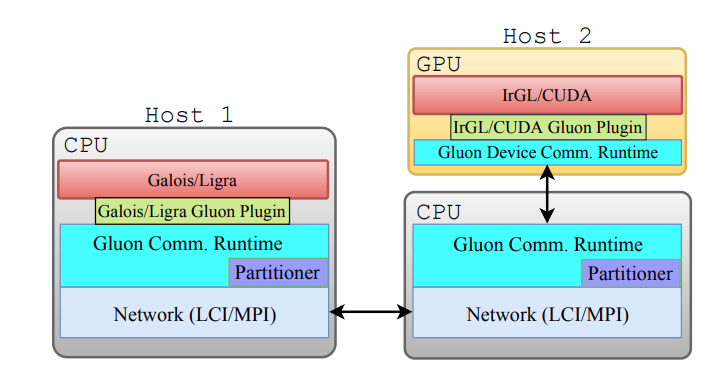
\includegraphics[width=0.49\textwidth]{gluon.png}
\mycaption{Gluon Overview}{The figure provides an overview of the Gluon Communication Substrate. 
}
\label{fig-gluon}
%\vspace{-20pt}
\end{figure}

D-IrGL is a distributed multi-GPU graph analytical framework. It supports multi-host multi-GPU architectures. D-IrGL uses the IrGL compiler for performing computations on each partition independently, and then uses the Gluon communication substrate for communicating and synchronizing data between the different GPUs. The performance of D-IrGL for different graphs depends mainly on the performance of the Gluon communication substrate. Figure~\ref{fig-gluon} shows the basic overview of the Gluon communication substrate. 

The limitation in the current Gluon implementation is that it does not use the features that are available in modern GPU architectures such as asynchronous data transfers, unified memory, or direct GPU-GPU communication without the involvement of CPUs. Since these features are independent of the graphs themselves, accommodating these features inside Gluon will improve the performance of all the graphs that use Gluon for communication. In this project, we  investigate the different features that have been added to the recent NVIDIA GPUs, and we attempt to apply them to the Gluon substrate and evaluate the performance of a simple BFS push algorithm for large graphs. 

The contributions that we make in this project are as follows:
\begin{enumerate}
\item We use streaming transfers of data between GPU and CPU of a node to overlap computation of data at the GPU along with communication of data between different nodes via CPU. 
\item We use Unified Virtual Addressing (UVA) to store the data of the graphs, to store larger partitions on each node. 
\item We attempt to implement inter-GPU communication of graph data without the involvement of CPU, among the GPUs located in a single machine as well as GPUs located across multiple machines. 
\end{enumerate}

\section{Overlapping Data Transfers}
\label{sec-async}

In this section, we talk about the details of streaming data transfers. Then we go on and talk about how we implement the streaming transfers in Gluon. We then discuss about the implementation and the challenges that we faced during the implementation. 

\subsection{Streaming Data Transfers}

A stream in CUDA is a sequence of operations that execute on the device in the order in which they are issued by the host code. While operations within a stream are guaranteed to execute in the prescribed order, operations in different streams can be interleaved and, when possible, they can even run concurrently. All device operations (kernels and data transfers) in CUDA run in a stream. When no stream is specified, the default stream (also called the “null stream”) is used. The default stream is different from other streams because it is a synchronizing stream with respect to operations on the device: no operation in the default stream will begin until all previously issued operations in any stream on the device have completed, and an operation in the default stream must complete before any other operation (in any stream on the device) will begin.

\begin{figure}
\centering
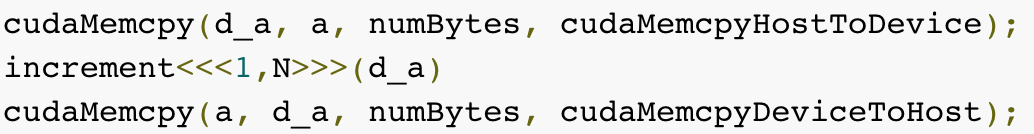
\includegraphics[width=0.49\textwidth]{async-serial.png}
\mycaption{}{This figure shows an algorithm for serially performing communication and computation. }
\label{fig-async-serial}
%\vspace{-20pt}
\end{figure}

\begin{figure}
\centering
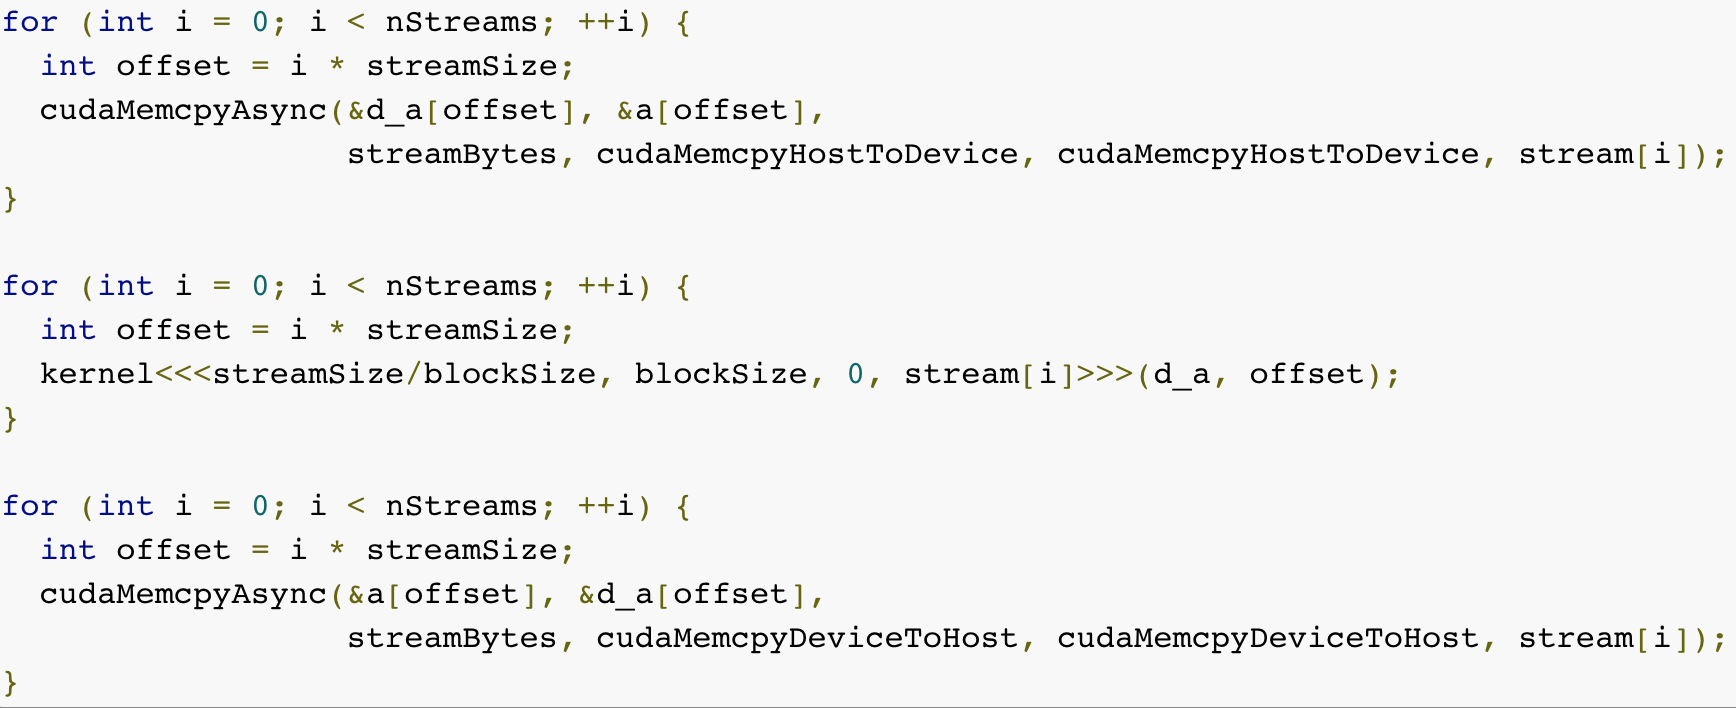
\includegraphics[width=0.49\textwidth]{async-parallel.png}
\mycaption{}{This figure shows an algorithm for overlapping communication and computation. }
\label{fig-async-parallel}
%\vspace{-20pt}
\end{figure}

The main goal behind streaming data transfers is that we want to overlap kernel execution along with data transfers. For this to be successful, the kernel execution and the data transfer should both occur in different, non-default streams. Also, the host memory that is involved in streaming data transfers should be pinned memory, if we want to achieve maximum performance. Figure ~\ref{fig-async-serial} shows the algorithm that uses default stream, which does not overlap computation with communication, whereas Figure~\ref{fig-async-parallel} shows the same algorithm that overlaps computation with communication using non-default streams. Note that both the algorithms provide current results, but the performance varies significantly. 

\begin{figure}
\centering
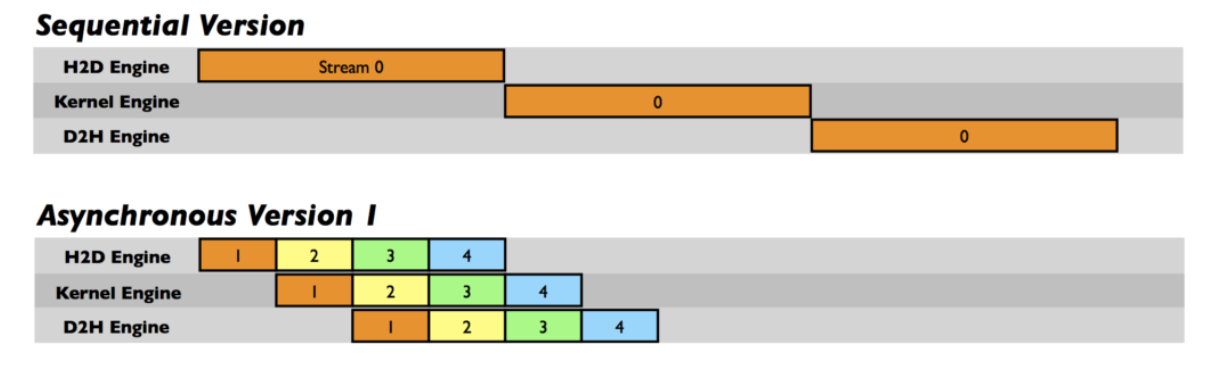
\includegraphics[width=0.49\textwidth]{async-perf.png}
\mycaption{Streaming data performance}{This figure shows the difference in performance between serial and overlapping communication with computation }
\label{fig-async-perf}
%\vspace{-20pt}
\end{figure}

Figure~\ref{fig-async-perf} shows the execution timelines for the sequential algorithm versus the asynchronous algorithm that overlaps computation with communication. As we can see from this figure, the end-to-end latency of the sequential version is roughly 2X compared to the asynchronous version. 

\subsection{Asynchronous Transfers in Gluon}

In the Gluon substrate, during the communication of graph data from a source node (or master node) to a destination node (or mirror node), the following steps take place, in a sequential order:
\begin{enumerate}
\item The offset data of the graph and the bitset data of the graph are computed at the GPU of the source
\item The offset data, bitset data and the shared graph data are copied and serialized into a CPU buffer at the source
\item The CPU buffer is transferred from the source to the destination
\item The CPU buffer at the destination is deserialized and copied to the GPU at the destination
\item The corresponding graph data, offset data and bitset data is computed at the GPU of the destination
\end{enumerate}

We modified these steps that occur during the synchronization phase, and we overlapped the computations in step 1 at the source with the data copy from GPU to CPU in step 2 using asynchronous streaming transfers. At the destination, we overlapped the data copy from CPU to GPU in step 4 with the computation on the copied data in step 5 using asynchronous streaming transfers. 

\subsection{Discussion}

The first challenge that we faced while applying this was to find out exactly where it is possible to apply this optimization in the large code base. We solved this by taking an example of the bfs\_push algorithm that is currently used for communicating the updates of a node in a graph to all its neighbors. Finally we found the point where there were transfers happening between GPU and CPU at the sender and the receiver, and we found opportunity to use this optimization in that part. We believe that it might be possible to apply this optimization to other parts of Gluon too, and this is just our prototype implementation of overlapping data transfers. 

The second challenge was regarding the use of pinned memory for achieving the asynchronous transfers. One limitation of pinned memory is that pinned memory cannot be reallocated or resized once it is allocated. This is an important problem because, in the case of sparse graphs, there is freq	uent resizing of buffers in Gluon, and it is impossible to know the size of the graphs or the number of bits in the bitset and offset to statically determine the size of the buffers. We could not use pinned buffers for this feature, and hence we believe that it won't lead to maximum performance improvements on large graphs. There needs to be a comprehensive change in the code base of Gluon to use pinned memory during the transfers, which might lead to better performance. 





\section{Unified Virtual Addressing}
\label{sec-uva}

In this section, we talk about the Unified Virtual Addressing (UVA) feature that we use to provide the same virtual memory for both GPU and CPU data, in order to have larger partitions of a graph per GPU. We first talk about the concept of UVA, and then we talk about how we implemented UVA in Gluon and finally we talk about the limitations and future directions with respect to this optimization. 

\subsection{UVA concept}
\begin{figure}
\centering
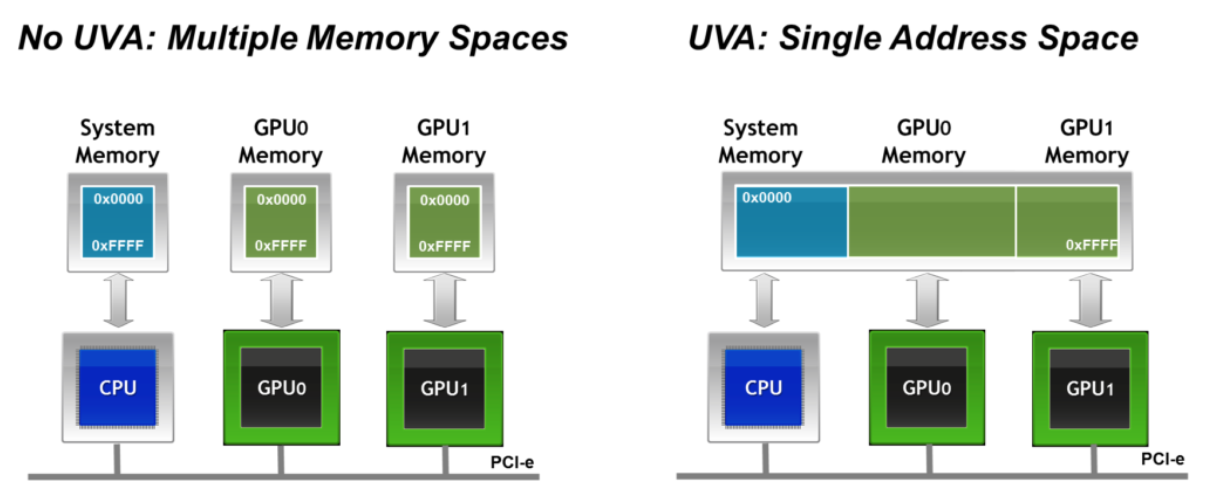
\includegraphics[width=0.49\textwidth]{uva-fig.png}
\mycaption{Unified Virtual Address}{The figure shows the address spaces with and without using UVA. 
}
\label{fig-uva}
%\vspace{-20pt}
\end{figure}

The GPU memory on servers is typically very limited. So storing graphs in GPUs places a limitation on the size of the graph per node, and requires larger clusters, increasing communication overhead and thus loss in performance. Furthermore, if we store the graphs on the host memory, then we need to copy the graphs from host memory to GPU memory and back during processing, as the address spaces of GPU memory and host memory are different. This leads to complicated implementations, and also cause overheads due to copying of data frequently between the host memory and GPU memory. To avoid this cost of copying and to store large graph partitions per GPU, NVIDIA introduced Unified Virtual Addresses (UVA). In UVA, both the GPU and the CPU memory lie in the same address space. The programmer does not need to worry about creating separate buffers for host memory and GPU memory. This is shown in Figure~\ref{fig-uva}. 

In UVA, memory is allocated in a region on the host using a call called cudaHostAlloc(). This memory is pinned memory, and cannot be paged out by the virtual memory system. Once the memory is allocated, it can be accessed from CPU as well as GPU. Note that the access of this pinned memory from GPU can be done without any copying of data from host to GPU. GPU threads can directly access and process data located in the pinned memory on the host. This technique allows you to leverage host memory when your device has limited global memory and also allows you to explicitly transfer data between host and device. 

However, sharing zero-copy memory data between host and device involves synchronizing memory accesses across host and device, because modifying data in zero-copy memory simultaneously from host and device could lead to undefined behavior. 

\subsection{Using UVA in Gluon}
We explore the use of UVA in the Gluon substrate in this project. In the original implementation of Gluon, the graph data as well as bitset and offset data is all present in the device memory. So we can imagine that for large graphs, this would lead to a problem, since the device (GPU) memory is very limited. We used Unified Virtual Addressing in which we allocated a the graph, and bitset and offset data on the host memory using cudaHostAlloc(). We then managed to use this pinned data that was allocated in the host directly for performing GPU computations, with a unified virtual address. We tested our implementation on a server with 2 GPUs, each containing 8GB of device memory. The host itself had 190GB memory. So we could potentially store 10x larger partitions on the host, as opposed to storing the graphs and the bitset and offset data entirely in the GPU. 

\subsection{Discussion and Limitations}
We stored the entire graph and all the bitset and offset data on the host memory using cudaHostAlloc(). Note that this leads to a non-trivial performance drop, since each node has to be fetched from the host through the PCI interface, instead of accessing from the fast bandwidth device memory. There is a lot of opportunity to explore smarter strategies to place only some parts of the graph which might be cold regions that are not accessed frequently using UVA, and store the hot regions in device memory. This would help us get the best of both worlds: get the high performance of device memory and also get the extra capacity from the host memory. 

Newer GPUs also support a mode called Unified Memory, which is different from Unified Virtual Addresses. The GPUs that we tested on did not have support for Unified Memory. In Unified Memory, the programmers get a similar interface as that of UVA with a single virtual address space for host and device memory. However, unified memory leads to better performance by transferring data from the host to the device when the device needs it, and managing the synchronization with the host copy of the data transparently without any efforts by the programmer. This has potential to improve the performance significantly by using smart prefetching and readahead strategies to improve the locality of data, and also gain the high capacity of host memory. 
\section{Inter-GPU communication without CPU Intervention}
In this section, we talk about GPUDirect technology for communicating between GPUs without any CPU intervention via Remote Dynamic Memory Access (RDMA). Then we talk about our attempt to implement the GPUDirect technology in the Gluon communication substrate.
We further discuss about the challenges that we faced in this implementation and conclude this section with our insights. 

\subsection{GPUDirect Technology}
Message Passing Interface (MPI) is a standard API for data communication using messages among distributed processes
and commonly used in High Performance Computing (HPC).
The MPI standard defines various message-passing techniques which covers from point-to-point messages to collective operations like broadcastings. 

\begin{figure}
\centering
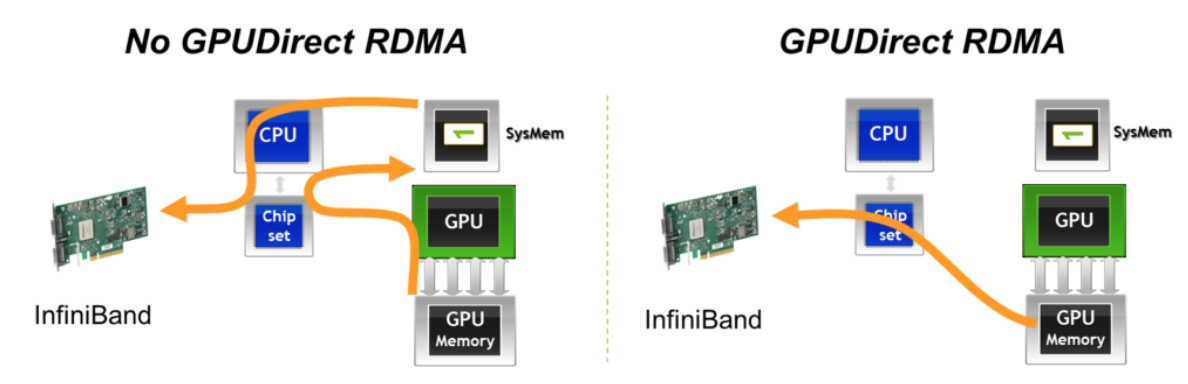
\includegraphics[width=0.49\textwidth]{gpu-rdma.png}
\mycaption{GPUDirect RDMA}{The figure shows the data transfers with and without GPUDirect RDMA. 
}
\label{fig-rdma}
%\vspace{-20pt}
\end{figure}

\begin{figure}
\centering
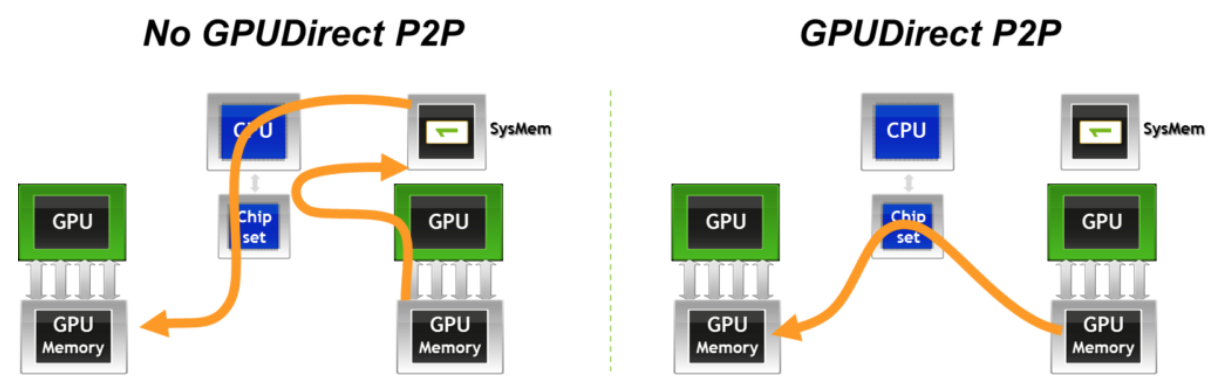
\includegraphics[width=0.49\textwidth]{gpu-ptp.png}
\mycaption{GPUDirect Peer-to-Peer}{The figure shows the data transfers with and without GPUDirect Peer-to-Peer. 
}
\label{fig-ptp}
%\vspace{-20pt}
\end{figure}


NVIDIA GPUDirect technologies provide high-bandwidth, low-latency communications with NVIDIA GPUs.
Remote Direct Memory Access (RDMA) is one of the newest GPUDirect technology which allows GPUs to
send its data directly to a network adapter without host memory participation. This is shown in Figure~\ref{fig-rdma}.
Another variant of this is Peer-to-Peer (P2P) transfers, which can accelerate intra-node communication.
Buffers can be directly copied between the memory of multiple GPUs in the same system through GPUDirect P2P. This is shown in Figure~\ref{fig-ptp}. 
Note that GPUDirectRDMA should exploit UVA technology; Otherwise, RDMA does not work since the MPI API calls on the host side cannot
recognize and point to GPU address.
GPUDirect technology also can be combined with other recent technologies such as asynchronous data transfer.

\subsection{GPUDirect in Gluon}
We attempted to implement the GPUDirect P2P and GPUDirect RDMA transfers on the Gluon Substrate
to accomplish direct inter-GPU communications without the host.
To support this functionality, we only aim for round based bfs\_push of lonestardist.
Gluon code is enormous and only for the one application, we had to modify entire execution paths of Gluon substrate.
The following lists show inter-GPU communication stages of the original Gluon.
\begin{enumerate}
\item Offsets and bitsets of the updated nodes are computed at the source GPU.
\item The computed data including the updated node label data are gathered, copied and serialized into a newly allocated CPU buffer.
\item The CPU buffer is transferred through asynchronous MPI APIs.
\item The sent CPU buffer is received at the destination CPU through asynchronous MPI APIs.
\item The received CPU buffer is deserialized and copied to the destination GPU.
\end{enumerate}
Using the GPUDirect Technology in this workflow, we can greatly reduce the overheads in these transfers, to the following steps:
\begin{enumerate}
\item Offsets and bitsets of the updated nodes are computed at the source GPU.
\item The computed date including the updated node label data are gathered, serialized and transferred directly from the source GPU using cuda-aware asynchronous MPI APIs supported by GPUDirect RDMA.
\item The sent data is directly received at the destination GPU using synchronous MPI.
\item The received data is deserialized and scattered to the proper locations. All of them are done on GPU.
\end{enumerate}
Note that all the steps can occur simultaneously along with other CPU computations. 
To do this, we also additionally apply asynchronous cuda memory copy with multiple streams, which avoids CPU blocking.
This feature, if applied effectively, has the potential to significantly improve the performance of data transfers, as compared to the other two features.

\subsection{Discussion and Limitations}
In this section, we introduce more detailed information about implementation.
The biggest challenge on this project was the current flow of MPI communications.
The following lists show how the current Gluon processes MPI messages. 
\begin{enumerate}
\item When Gluon substrate is initialized, the background thread called worker thread starts to run in background.
Until BFS finishes, the thread polls and catches all the OpenMPI messages received on the node.
\item All MPI message processings are done asynchronously.
If any message processing is done, then it moves to either receive vector or send vector.
Each vector comprises to buffer lists indexed by the host id. For example, the first item of the receive vector
contains buffer lists sent by the host 1.
\item For each round of BFS, the Gluon substrate enumerates the receive vector and checks whether any host sends 
message and the message is fully received ot not.
If it is, the substrate starts to process the received buffer. 
\end{enumerate}

All the above sequences are performed on \textit{CPU}.
However, GPUDirect messages should be received by GPU, not CPU.
To do this, GPU buffers should be preallocated before message receives with proper size, and 
gathered by the worker thread.
In addition, we need a GPU vector type to store and handle send and receive messages invoked dynamically. 
We can reuse the current Gluon network system in the future, but for this project, 
we just focused on the basic GPUDirect RDMA supports.
First, we use one fixed tag, 10000, for OpenMPI GPUDirect messages and make the worker thread ignore them.
Second, we remove the original serialization/deserialization/copy/scatter codes for CPU-GPU communications and 
replace them to GPU-GPU gather and scatter communications. In this case, we also serialize and deserialize 
message in order to avoid complex network system. But it is done only on GPU, not CPU.
Finally, the main thread requests MPI send or receive the serialized buffer messages, not the worker thread.

Our current implementation is the first attempts to support GPUDirect techniques on Gluon.
Therefore, it has several limitations, but also implies that there are lots of rooms for improvements.
First, since we could not collect GPU data to be sent or to be received, due to the shortage of 
stable GPU vector type, we only aimed for one-to-one GPU communication.
Therefore, in the future, we could improve and extend the current communication between two GPUs to multiple GPUs communication.
Second, we use asynchronous MPI send and synchronous MPI receive.
Using asynchronous MPI receive would improve performance.
This is also doable after we make GPU vector. As the original Gluon network does, 
asynchronous messaging would be processed in the background.
Third, GPUDirect RDMA can easily apply future optimizations of other techniques such as locality-aware memory management,
memory reuse and pinned memory.

\section{Evaluation}
\label{evaluation}
All tests were done on an Tuxedo which has one node with 4 K80 GPUs and 2 GTX 1080 GPUs.
We use distributed push-style and round based bfs of lonestardist. For input graphs, we used 
social network graph, twitter40 and road network, road-USA. The former represents 
performance of power-law graph and the latter represents performances of large dimater graph. 
For UVA and asynchronous memory copy, we used two GPUs within single node and 
for GPUDirect, we tested two GPUs and six GPUs within single node separately in order to understand
network communication overheads.

\subsection{Asynchronous memory copy}
%The table X shows comparsion between synchronous and asynchronous memory copy.
Twitter with asynchronous memory copy shows 14.1 seconds and with synchronous memory copy shows 
14.3 seconds. Road-network with asynchronous memory copy shows 385 seconds and 
with synchronous memory copy shows 391 seconds.
For all input graphs, we only got from 1 to 2 percent improvements.
This is because our projects only aim to overlap GPU-CPU and CPU-CPU memory copy.
Moreover, we are using page-able memory which is managed by kernel.
We expect taht we can improve this performance further by utilizing pinned memory and overlapping 
timelines of memory copy and computation parts.

\subsection{UVA}
Twitter with UVA shows 31 seconds and without UVA shows 14 seconds.

\subsection{GPUDirect: RDMA and p2p copy}
Twitter with the combination of RDMA, UVA and asynchronous copy, and 6 nodes shows 14 seconds
but with the original one shows 40 seconds. 
As the network amoung is increased, we could accomplish faster performance since 
we can remove CPU-GPU copies.

\section{Conclusion}
We explored the use of different powerful features that are present in modern GPU architectures and applied them to D-IrGL. We faced interesting challenges in implementing them and also got ideas for several interesting directions for future work. We hope that the contributions of the project will prove to be valuable additions in the Gluon communication substrate and will improve the performance of distributed graph analytics frameworks significantly. 
%\section{Introduction}

%Text of paper \ldots


%% Acknowledgments
\begin{acks}                            %% acks environment is optional
                                        %% contents suppressed with 'anonymous'
  %% Commands \grantsponsor{<sponsorID>}{<name>}{<url>} and
  %% \grantnum[<url>]{<sponsorID>}{<number>} should be used to
  %% acknowledge financial support and will be used by metadata
  %% extraction tools.
  We would like to thank Prof. Keshav Pingali for helping us to acquire the required background knowledge for this project through the course. We would also like to thank our project leaders Vishwesh Jatala and Roshan Dathathri for always being available to help us throughout the project. We would finally like to thank everyone else who directly and indirectly helped us achieve our goals of the project. 
\end{acks}
}

\newpage

\bibliographystyle{ACM-Reference-Format}
\bibliography{all}

%% Bibliography
%\bibliography{bibfile}


\end{document}
